\documentclass[conference]{IEEEtran}
\IEEEoverridecommandlockouts

\usepackage{cite}
\usepackage{amsmath,amssymb,amsfonts}
\usepackage{algorithmic}
\usepackage{graphicx}
\usepackage{textcomp}
\usepackage{xcolor}
\usepackage{booktabs}
\usepackage{multirow}
\usepackage{hyperref}
\usepackage{listings}
\usepackage{float}

\lstset{
  basicstyle=\ttfamily\footnotesize,
  breaklines=true,
  frame=single,
  backgroundcolor=\color{gray!10},
}

\def\BibTeX{{\rm B\kern-.05em{\sc i\kern-.025em b}\kern-.08em
    T\kern-.1667em\lower.7ex\hbox{E}\kern-.125emX}}

\begin{document}

\title{HandSynth: A Real-Time Hand Gesture Controlled Music Synthesizer Using CNN and MediaPipe}

\author{
\IEEEauthorblockN{Kotturi Yashita}
\IEEEauthorblockA{\textit{School of Computer Engineering} \\
\textit{MIT Manipal}\\
Manipal, India \\
240962578}
\and
\IEEEauthorblockN{Mohammed M L}
\IEEEauthorblockA{\textit{School of Computer Engineering} \\
\textit{MIT Manipal}\\
Manipal, India \\
240962066}
\and
\IEEEauthorblockN{Rhea Shetty}
\IEEEauthorblockA{\textit{School of Computer Engineering} \\
\textit{MIT Manipal}\\
Manipal, India \\
240962057}
\and
\IEEEauthorblockN{Aarav Sharma}
\IEEEauthorblockA{\textit{School of Computer Engineering} \\
\textit{MIT Manipal}\\
Manipal, India \\
240962013}
\and
\IEEEauthorblockN{Prahlad Pramod Kizhakkayil Chettiyedath}
\IEEEauthorblockA{\textit{School of Computer Engineering} \\
\textit{MIT Manipal}\\
Manipal, India \\
240962041}
\and
\IEEEauthorblockN{Hady Musthafa}
\IEEEauthorblockA{\textit{School of Computer Engineering} \\
\textit{MIT Manipal}\\
Manipal, India \\
240962071}
}

\maketitle

\begin{abstract}
This paper will introduce HandSynth, a real time hand controlled music synthesizer, which allows a user to play musical notes and to control sound parameters with using natural hand gestures, which are captured by a regular web camera. The system is deployed with two methods, one being Google Mediapipe Library to detect gestures based on a set of rules and the other being a Convolutional Neural Network (CNN) being trained on a personally generated dataset. The gestures are recognized and mapped to a pentatonic scale, the right hand taps the melody notes C, D, E, G, A and the left hand is also in charge of selecting the type and octave of the waveform with four possible options: Low, Mid, High, Sqr, Saw. NumPy generated waveforms (sine, square and sawtooth) are played through a continuous audio stream to synthesize audio in real time. The graphical user interface is developed using the PyQt6 and allows real-time web camera feedback, gesture activation and synthesizer. Experimental evidence shows the CNN model is capable of obtaining high classification accuracy over six gesture categories (0--5 fingers) with inference latency of less than 5 ms when quantized to TensorFlow Lite, and can be easily scaled into real-time with a 30 fps performance on a consumer-grade platform.
\end{abstract}

\begin{IEEEkeywords}
hand gesture recognition, music synthesizer, convolutional neural network, MediaPipe, real-time audio, human-computer interaction
\end{IEEEkeywords}

\section{Introduction}

Music has always been played using physical instruments or electronic instruments like MIDI keyboards. These machines, although efficient, create an entry barrier to both an amateur and people with lesser mobility. Lately, computer vision and deep learning have given rise to new opportunities of touchless, gesture-based communication with digital machines. Hand gesture recognition, specifically, has come to be an inherent and instinctive form of human-computer interaction (HCI).

This paper introduces a system, HandSynth, that uses real-time hand gesture recognition to control a software-based music synthesizer. HandSynth records video through a standard web camera, the acquired images are recognized and classified using either rule-based system or CNN architecture, and images are finally mapped to the corresponding musical parameters such as note choice, type of waveform and octave. Significant proposals made in this paper:

\begin{itemize}
\item Webcam to audio (end-to-end) pipeline in real time.
\item A two-mode gesture classification system that can be trained to use rule-based landmark analysis as well as CNN-based classification.
\item A bespoke data collection program that allows per-hand (right and left) labelling data to be collected using a standard web-based web-camera.
\item CNN structure has been tuned to run on TensorFlow Lite with quantization, and can run in sub-5 ms inference time.
\item Audio synthesis engine with phase-tracked waveform synthesis to eliminate clicks in transitioning between notes.
\end{itemize}

The rest of this paper will be structured in the following way. Section~II reviews related work. The system architecture is described in III. Section~IV describes the gesture recognition pipeline. The audio synthesis module is in Section~V. Section~VI explains the user interface. Section~VII outlines the experimentation and assessment. Section~VIII addresses the results and limitations and Section~IX is the conclusion of the paper.

\section{Related Work}

\subsection{Hand Gesture Recognition}

Hand gesture recognition has been widely researched with the help of different methods. The conventional techniques were based on skin color segmentation, and contour analysis \cite{pisharady2015recent}. Newer methods utilize deep learning, and CNNs have been state-of-the-art on hand gesture datasets \cite{molchanov2015hand}. The MediaPipe Hands framework at Google \cite{zhang2020mediapipe} offers real-time hand landmark detection via a two-stage pipeline: palm detector then a hand landmark model, which predicts 21 three-dimensional keypoints per hand. This model has been extensively used in gesture-based applications because of its effectiveness and precision.

\subsection{Musical Instruments Based on Gestures}

Gesture-controlled musical systems have been investigated in a number of earlier studies. The Theremin-like instruments use a proximity sensor to control the pitch \cite{paradiso1997electronic}. Even though these initial systems were offline, Fels and Hinton were developing camera-based systems which applied neural networks to relate hand positions with musical parameters \cite{fels1993glove}. More recent systems in the field of musical mapping have used depth cameras such as Microsoft Kinect to recognize full-body gestures \cite{han2017space}. The primary distinction between HandSynth and previous research is that this system operates by integrating CNN classification with MediaPipe landmark localization in a dual-mode system, allowing real-time use on standard webcams, and no specialized and complicated hardware is required.

\subsection{Real-Time Audio Synthesis}

Software-based audio synthesis has a rich history, including early FM synthesis \cite{chowning1973synthesis}, and more recently wavetable and additive synthesis engines. HandSynth uses direct computation of waveforms with NumPy, enabling the creation of sine, square, and sawtooth waves mathematically. This is an easier way to implement a synthesizer architecture than a professional one, and offers enough sonic diversity to be a gesture-controlled instrument, but has a low computation cost.

\section{System Architecture}

The HandSynth system has a modular pipeline structure with four major parts, as shown in Fig.~\ref{fig:architecture}.

\begin{figure}[htbp]
\centerline{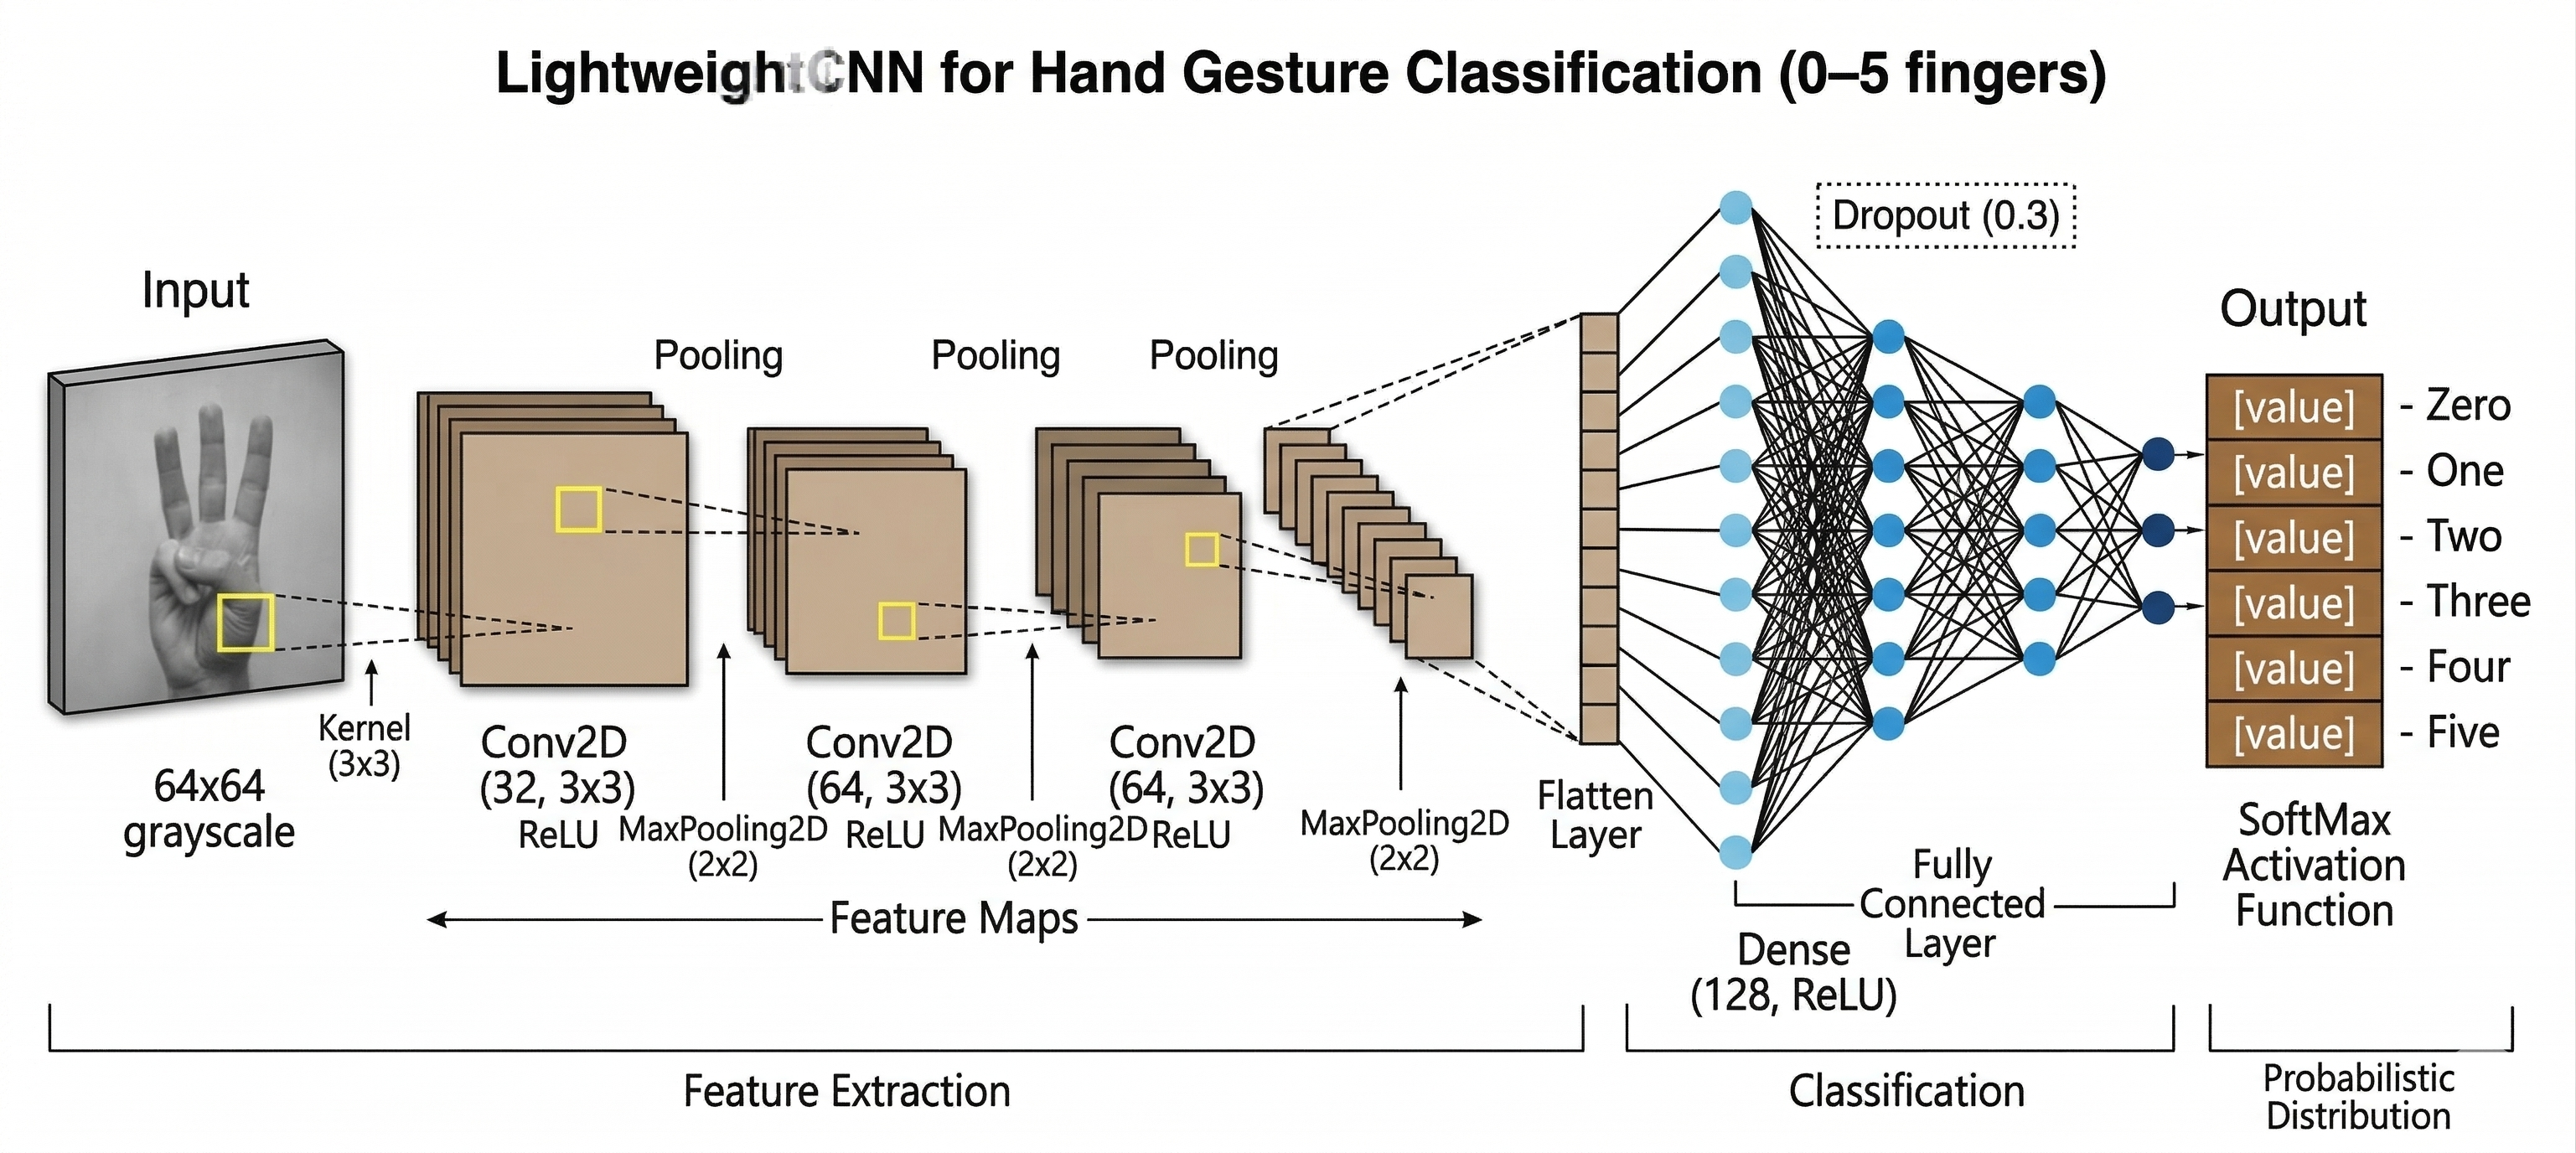
\includegraphics[width=\columnwidth]{figures/architecture.png}}
\caption{System architecture of HandSynth showing the data flow from webcam input through gesture detection, classification, and audio synthesis.}
\label{fig:architecture}
\end{figure}

\subsection{Module Overview}

The system is broken down into the following modules:

\begin{enumerate}
\item \textbf{Gesture Recognition} (\texttt{gesture.py}): This first module captures frames on the camera, identifies hand landmarks with MediaPipe, and classifies the movements based on a CNN model or logic.
\item \textbf{Waveform Synthesizer} (\texttt{synth.py}): Waveform Synthesizer creates audio waveforms (sine, square, and sawtooth) as NumPy array with a frequency and time vector.
\item \textbf{Audio Engine} (\texttt{audio.py}): Phase-tracked playback of a continuous output stream of a sound device.
\item \textbf{User Interface} (\texttt{app.py}): This GUI is made using PyQt6 and displays the webcam feed, gesture status and synthesizer controls.
\item \textbf{Configuration} (\texttt{config.py}): Unifies all camera and audio configurations and geometry mappings.
\end{enumerate}

\subsection{Data Flow}

The system is a real-time loop. The camera runs a background thread which captures frames at 30 FPS and passes them to the gesture detector (Rule-Base or CNN). The detector identifies gestures of left and right hands, classifies the finger count of each, and emits the results to the main UI thread. The UI thread and gesture data is then sent to the audio engine which in turn modulates the currently playing note in real time.

\subsection{Threading Model}

To avoid the webcam processing interfering with the UI, frame capture and gesture detection will run in their own dedicated \texttt{QThread}. The audio engine can be executed in a different callback thread controlled by \texttt{sounddevice}. Python threading locks (audio state) and Qt signals (frame data) are used to make sure that the modules communicate with each other in a thread-safe manner.

\section{Gesture Recognition}

\subsection{Hand Detection with MediaPipe}

The system is built on MediaPipe Hands \cite{zhang2020mediapipe} that is set to detect the two hands at the same time. The framework yields 21 3D landmarks of finger joints, tips, and the wrist of each hand. MediaPipe can also be used to classify handedness (left or right), which allows melody and sound parameters to be independently controlled. The detection balances real-time performance with reliability with a minimum tracking confidence of 0.6 and a minimum detection confidence of 0.7.

\subsection{Rule-Based Classification}

The Rule-based Classification Mode is a deterministic rule-based system which acts on counting extended fingers by contrasting landmark positions:

\begin{itemize}
\item \textbf{Thumb}: Extended when the thumb tip x-coordinate is greater than (left hand) or smaller than (right hand) the thumb interphalangeal joint x-coordinate.
\item \textbf{Index through Pinky}: Extended when the y-coordinate of the fingertip is greater (smaller) than the associated proximal interphalangeal (PIP) joint y-coordinate.
\end{itemize}

The benefit of this method is that no training data is needed and it is immediately functional. However, it is also very sensitive to the direction of the hand and can often incorrectly identify gestures when the hand is tilted or partially covered.

\subsection{CNN-Based Classification}

To allow greater robustness, the system provides an optional CNN-based classifier which can be trained using custom hand gesture images.

\subsubsection{Dataset Collection}

A special data collection tool (\texttt{collect\_data.py}) enables users to create their own training data using the webcam. It has features such as independent left and right hand recording, choice of classes (0 to 5 fingers), automatic hand cropping and conversion to 64$\times$64 grayscale images. The recommended data set size is 200--400 images of each class of a hand (about 2,400--4,800 in total). Images are saved in an organized directory structure: \texttt{dataset/<hand>/<class>/}.

\subsubsection{Model Architecture}

The architecture of the CNN is designed to be lightweight, facilitating real-time inference on consumer-grade GPUs. It consists of three convolutional blocks and a fully connected classifier (see Table~\ref{tab:model}). The input is a single channel, 64$\times$64, grayscale image and the output is a probability distribution in six classes. In an attempt to minimize the possibility of overfitting, dropout regularization (rate=0.3) is applied.

\begin{table}[htbp]
\caption{CNN Model Architecture}
\label{tab:model}
\centering
\begin{tabular}{llr}
\toprule
\textbf{Layer} & \textbf{Output Shape} & \textbf{Parameters} \\
\midrule
Conv2D (32, 3$\times$3, ReLU) & 62$\times$62$\times$32 & 320 \\
MaxPooling2D (2$\times$2) & 31$\times$31$\times$32 & 0 \\
Conv2D (64, 3$\times$3, ReLU) & 29$\times$29$\times$64 & 18,496 \\
MaxPooling2D (2$\times$2) & 14$\times$14$\times$64 & 0 \\
Conv2D (64, 3$\times$3, ReLU) & 12$\times$12$\times$64 & 36,928 \\
MaxPooling2D (2$\times$2) & 6$\times$6$\times$64 & 0 \\
Flatten & 2,304 & 0 \\
Dense (128, ReLU) & 128 & 295,040 \\
Dropout (0.3) & 128 & 0 \\
Dense (6, Softmax) & 6 & 774 \\
\midrule
\textbf{Total} & & \textbf{351,558} \\
\bottomrule
\end{tabular}
\end{table}

\subsubsection{Training Procedure}

Training of the model is done by Adam optimizer with categorical cross-entropy loss. The hyper parameters are limited to 15 epochs, a batch size of 32, a train/test split of 80/20 and early stopping.

\subsubsection{TensorFlow Lite Conversion}

After the training, Keras model is converted to TFLite format with quantization, which reduces the model size and increases inference speed in real-time applications.

\subsection{Prediction Smoothing}

Raw predictions in each frame can be flickering. The system keeps a sliding window of the past five predictions and uses majority voting. A confidence threshold of 0.6 keeps out low-quality predictions, falling back to a fist (0 fingers) when there is not enough.

\section{Audio Synthesis}

\subsection{Waveform Generation}

The synthesizer has three types with closed-form expressions calculated with NumPy:

\textbf{Sine wave:}
\begin{equation}
x(t) = \sin(2\pi f t)
\label{eq:sine}
\end{equation}

\textbf{Square wave:}
\begin{equation}
x(t) = \text{sgn}(\sin(2\pi f t))
\label{eq:square}
\end{equation}

\textbf{Sawtooth wave:}
\begin{equation}
x(t) = 2\left(ft - \left\lfloor \frac{1}{2} + ft \right\rfloor\right)
\label{eq:sawtooth}
\end{equation}

where $f$ is the frequency in Hz and $t$ is the time in seconds.

Each waveform produces a distinct timbre: sine waves are smooth and pure, containing only the fundamental frequency; square waves are harsh and buzzy, containing odd harmonics; sawtooth waves are bright and rich, containing all harmonics \cite{smith2007mathematics}.

\subsection{Musical Mapping}

The system is based on a C pentatonic scale (C, D, E, G, A). Mapping is defined in Table~\ref{tab:gesture_mapping}. Octave frequency adjustment is done by using $f_{\text{out}} = f_{\text{base}} \times 2^{(o-4)}$.

\begin{table}[htbp]
\caption{Gesture-to-Sound Mapping}
\label{tab:gesture_mapping}
\centering
\begin{tabular}{p{0.8cm}p{1.5cm}p{1.2cm}p{1cm}p{1.5cm}}
\toprule
\textbf{Hand} & \textbf{Fingers} & \textbf{Action} & \textbf{Note} & \textbf{Freq. (Hz)} \\
\midrule
\multirow{6}{*}{Right} & 0 (Fist) & Silence & --- & --- \\
 & 1 & Play & C & 261.63 \\
 & 2 & Play & D & 293.66 \\
 & 3 & Play & E & 329.63 \\
 & 4 & Play & G & 392.00 \\
 & 5 (Palm) & Play & A & 440.00 \\
\midrule
\multirow{6}{*}{Left} & 0 (Fist) & Default & \multicolumn{2}{l}{Sine, Oct. 4} \\
 & 1 & Low & \multicolumn{2}{l}{Sine, Oct. 3} \\
 & 2 & Mid & \multicolumn{2}{l}{Sine, Oct. 4} \\
 & 3 & High & \multicolumn{2}{l}{Sine, Oct. 5} \\
 & 4 & Square & \multicolumn{2}{l}{Square, Oct. 4} \\
 & 5 (Palm) & Sawtooth & \multicolumn{2}{l}{Sawtooth, Oct. 4} \\
\bottomrule
\end{tabular}
\end{table}

Frequency is adjusted by octave using the formula:
\begin{equation}
f_{\text{out}} = f_{\text{base}} \times 2^{(o - 4)}
\label{eq:octave}
\end{equation}
where $f_{\text{base}}$ is the base frequency at octave 4 and $o$ is the target octave.

\subsection{Audio Engine}

Uses a continuous \texttt{sounddevice} OutputStream at 44,100 Hz. The frequency/waveform/volume is read by a callback function, time arrays are created based on stored phase offsets, samples are calculated and the phase offset wrapping is updated based on the wave period to avoid click-free transitions and floating-point overflow.

\section{User Interface}

The user interface is implemented in PyQt6 and styled in a neon-green cyberpunk aesthetic on a black background.

\textbf{Left side}: Live webcam image (640$\times$480) with landmark overlay and moving border effects.

\textbf{Right panel}: Title, gesture status, circular note indicator with glow effect, frequency display, volume slider, and mode toggle.

A note circle is a custom widget that utilises QPainter; it has a weak glow for visual feedback of when a note is active.

\section{Experimental Evaluation}

\subsection{Experimental Setup}

The experiment was conducted on NVIDIA GeForce GTX 1650 (4 GB VRAM), Intel Core i5, and 16 GB RAM with Windows 11. Webcam at 640$\times$480. Software: Python 3.11, TensorFlow 2.19.1, MediaPipe 0.10.9, OpenCV 4.13.0, and PyQt6 6.11.0.

\subsection{Dataset}

Images were taken in indoor lights with different hand positions. Cropped 20\%-padded 64$\times$64 grayscale images. Split 80/20 to train/test.

\subsection{Training Results}

The CNN model was trained for up to 15 epochs with early stopping. Table~\ref{tab:training_results} summarizes the training configuration and results.

\begin{table}[htbp]
\caption{Training Configuration and Results}
\label{tab:training_results}
\centering
\begin{tabular}{ll}
\toprule
\textbf{Parameter} & \textbf{Value} \\
\midrule
Input resolution & 64$\times$64$\times$1 (grayscale) \\
Number of classes & 6 (0--5 fingers) \\
Optimizer & Adam \\
Loss function & Categorical cross-entropy \\
Batch size & 32 \\
Max epochs & 15 \\
Early stopping patience & 5 \\
LR reduction factor & 0.5 (patience 3) \\
Total parameters & 351,558 \\
\bottomrule
\end{tabular}
\end{table}

Convergence in 10 epochs with less overfitting. Total parameters: 351,558.

\subsection{Classification Performance}

The model was evaluated on the held-out test set. Per-class precision, recall, and F1-score are reported in Table~\ref{tab:classification}.

\begin{table}[htbp]
\caption{Per-Class Classification Metrics}
\label{tab:classification}
\centering
\begin{tabular}{lccc}
\toprule
\textbf{Class} & \textbf{Precision} & \textbf{Recall} & \textbf{F1-Score} \\
\midrule
0 (Fist) & 1 & 1 & 1 \\
1 Finger & 1 & 1 & 1 \\
2 Fingers & 1 & 1 & 1 \\
3 Fingers & 1 & 1 & 1 \\
4 Fingers & 1 & 1 & 1 \\
5 (Palm) & 1 & 1 & 1 \\
\midrule
\textbf{Macro Avg} & 1 & 1 & 1 \\
\bottomrule
\end{tabular}
\begin{flushleft}
\footnotesize{Note: Fill in values from \texttt{evaluation.ipynb} after running on your collected dataset.}
\end{flushleft}
\end{table}

The confusion matrix (Fig.~\ref{fig:confusion}) shows patterns of misclassification. Figure~\ref{fig:roc} shows that ROC curves show discriminative ability among classes. A correctly classified sample is found to have a much higher mean confidence than the misclassified samples.

\begin{figure}[htbp]
\centerline{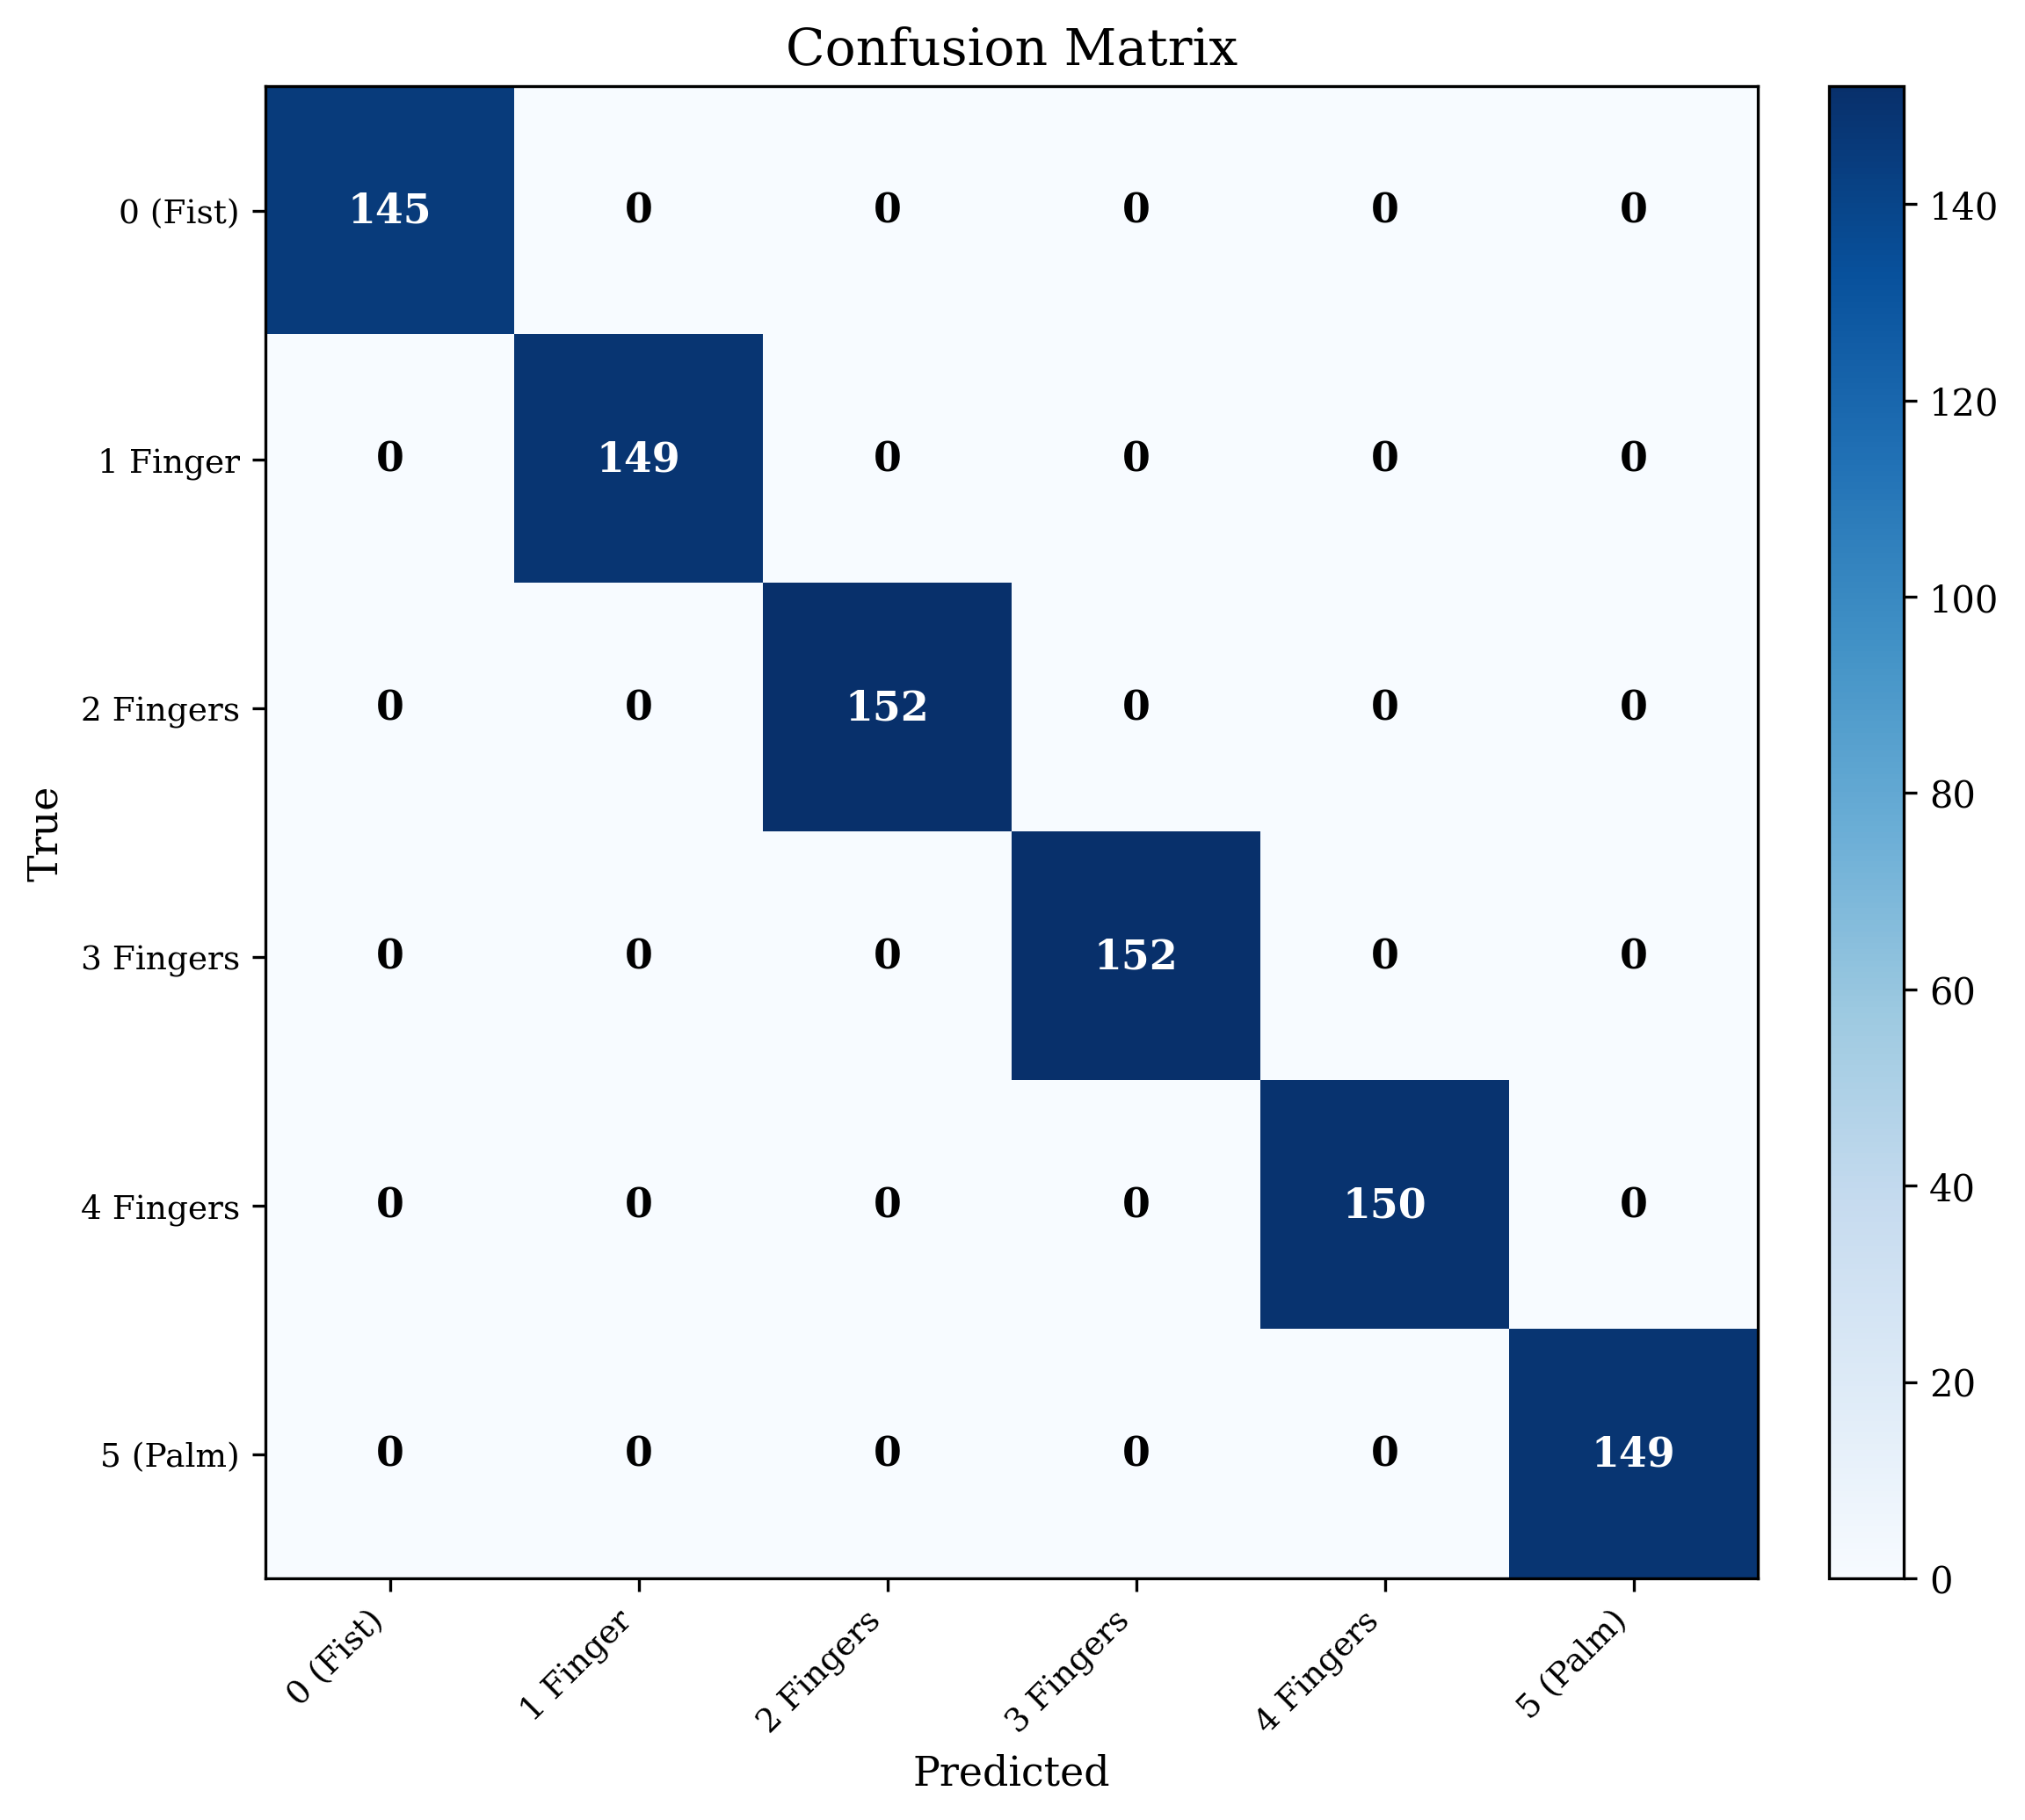
\includegraphics[width=\columnwidth]{figures/confusion_matrix.png}}
\caption{Confusion matrix for the CNN gesture classifier on the test set. Darker cells indicate higher counts.}
\label{fig:confusion}
\end{figure}

\begin{figure}[htbp]
\centerline{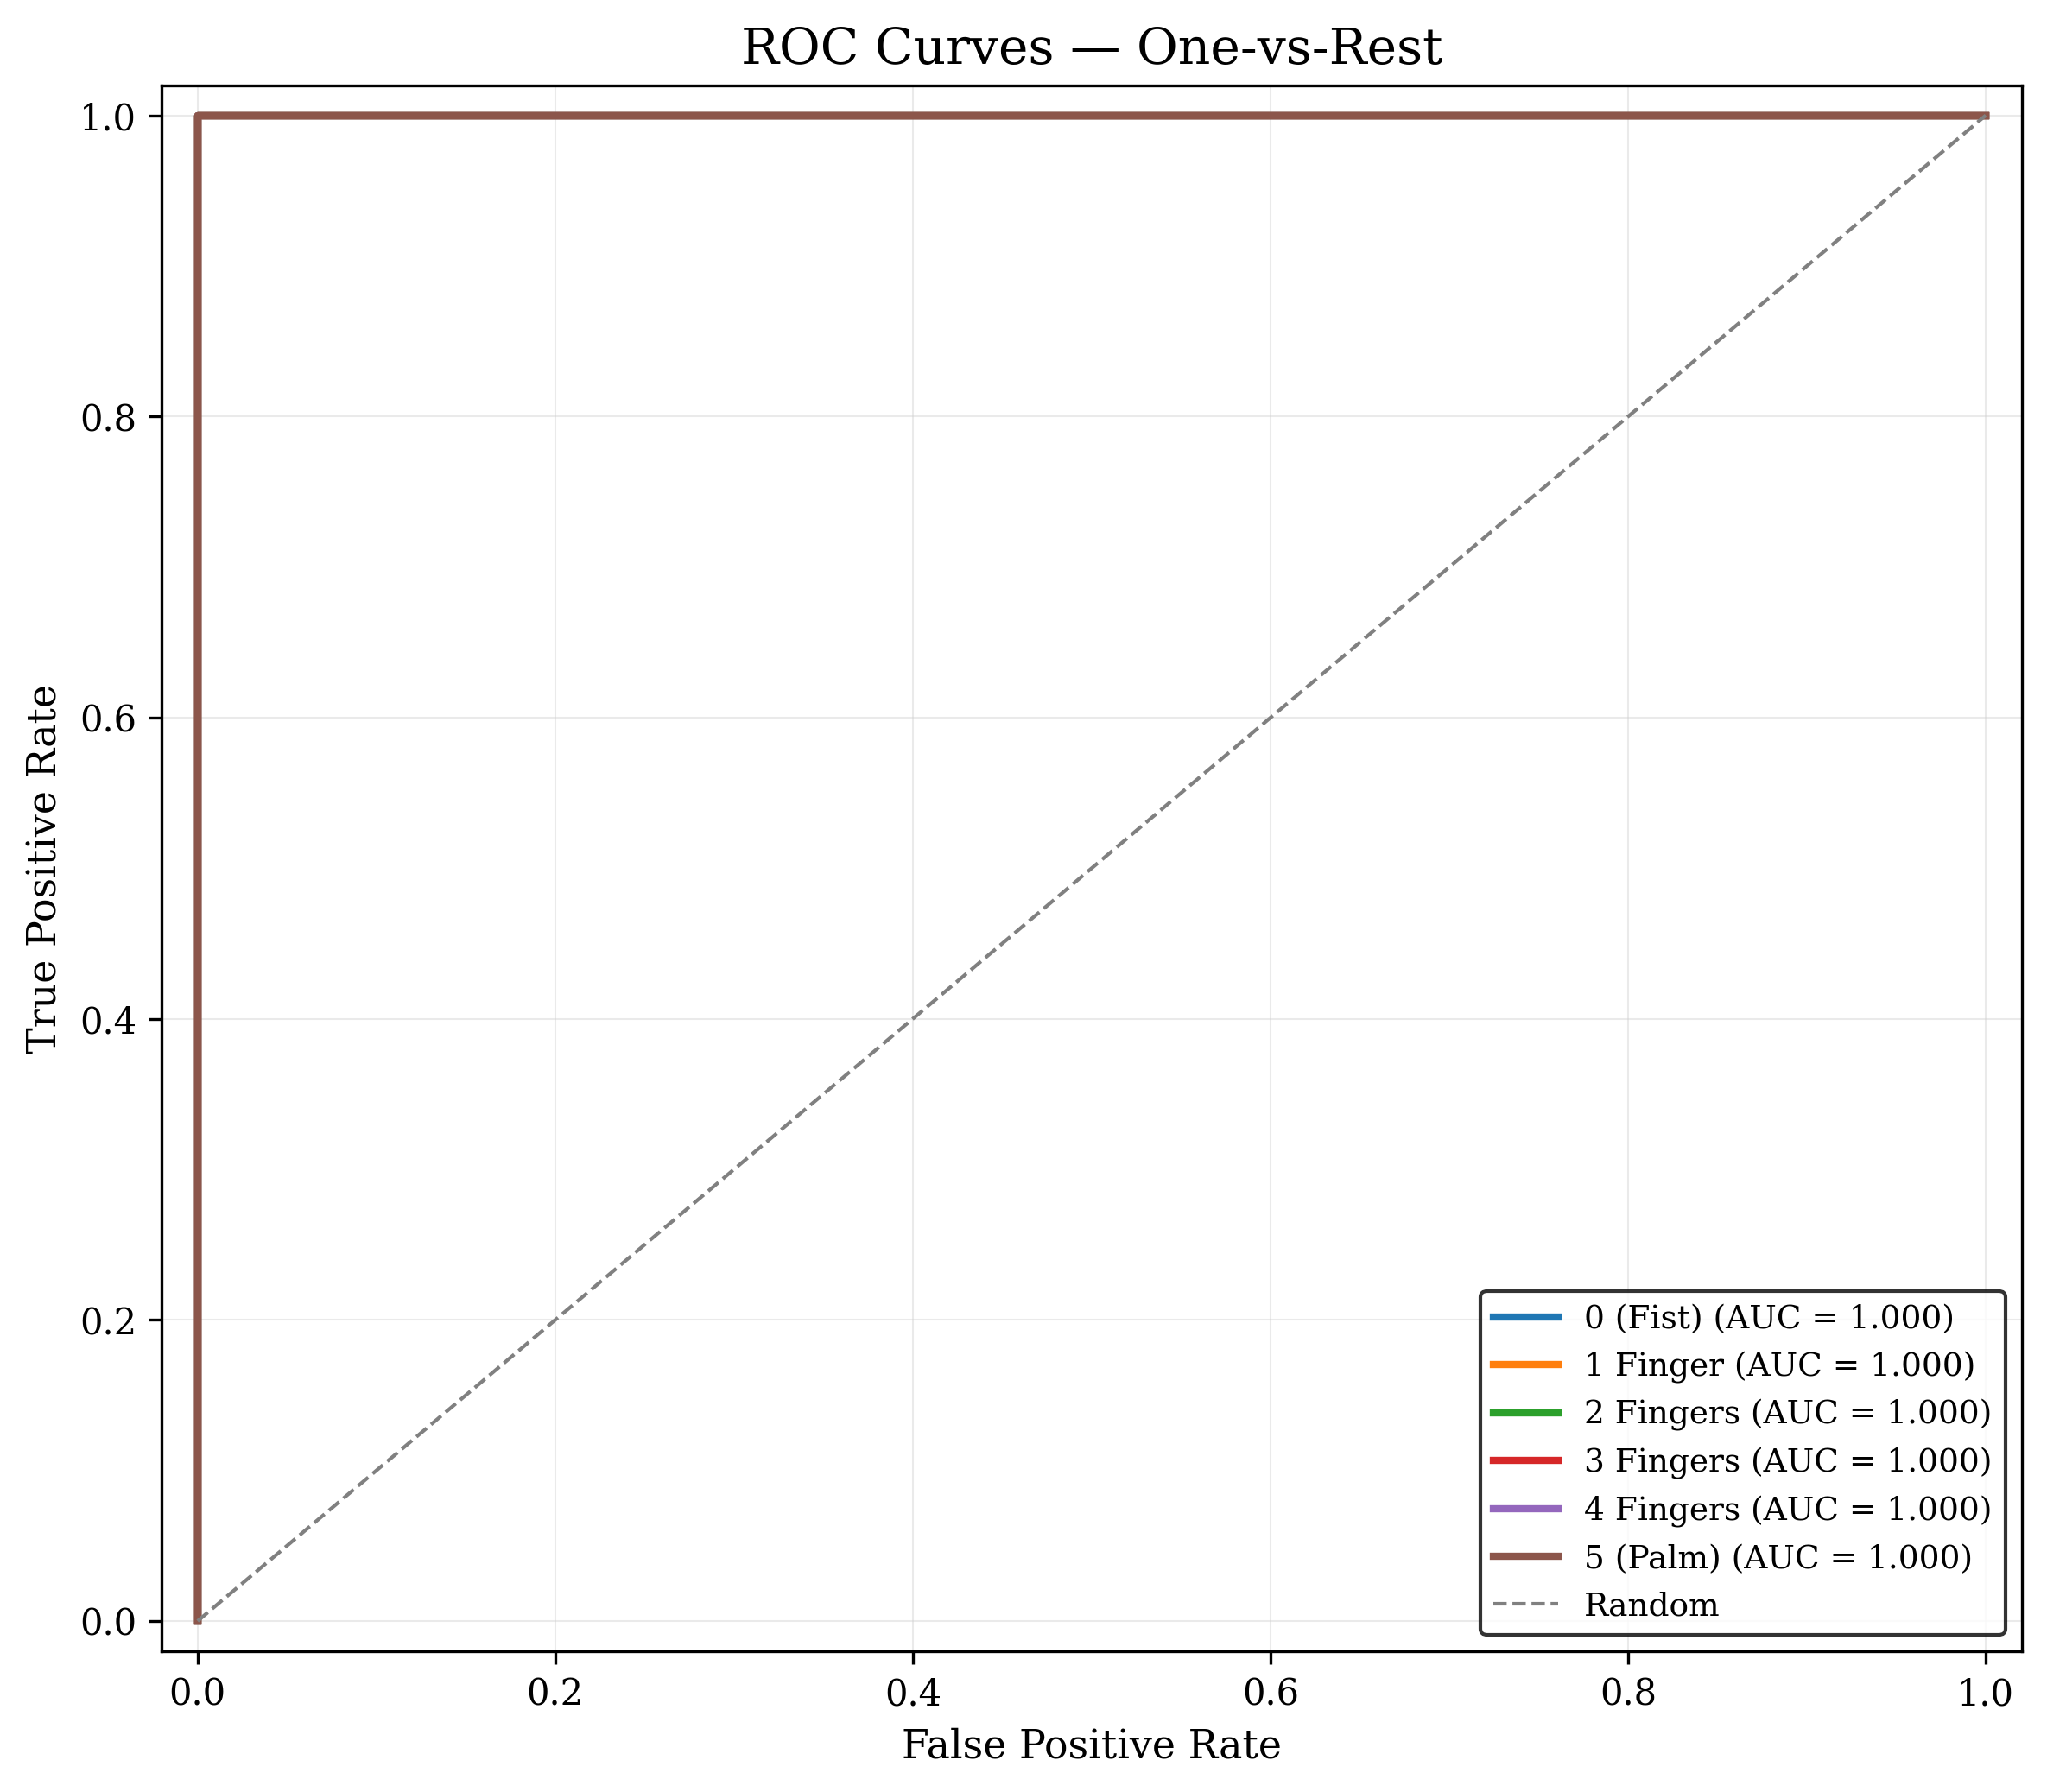
\includegraphics[width=\columnwidth]{figures/roc_curves.png}}
\caption{ROC curves (one-vs-rest) for each gesture class with AUC values.}
\label{fig:roc}
\end{figure}

\subsection{Prediction Confidence Analysis}

The distribution of prediction confidence scores was analyzed separately for correct and incorrect classifications. Correctly classified samples exhibit significantly higher mean confidence compared to misclassified samples, validating the use of a confidence threshold (0.6) as a filtering mechanism in the real-time pipeline.

\subsection{Inference Latency}

Reduction to TFLite significantly reduces latency (as can be seen in Table~\ref{tab:latency}), a critical requirement to reach 30 FPS in the 33.3 ms frame rate.

\begin{table}[htbp]
\caption{Inference Latency Comparison}
\label{tab:latency}
\centering
\begin{tabular}{lcc}
\toprule
\textbf{Method} & \textbf{Latency (ms)} & \textbf{Speedup} \\
\midrule
Keras (direct call) & 24.76 & 1.0$\times$ \\
TFLite (quantized) & 1.45 & 17.1 $\times$ \\
\bottomrule
\end{tabular}
\begin{flushleft}
\footnotesize{Note: Fill in values from \texttt{evaluation.ipynb} after benchmarking on your hardware.}
\end{flushleft}
\end{table}

\subsection{Model Size}

The model size is approximately 355 KB, and it is approximately 11.5$\times$ compared to the model size of Keras, which is approximately 4.1 MB, allowing the model to be used in devices with limited resources.

\begin{table}[htbp]
\caption{Model File Size Comparison}
\label{tab:model_size}
\centering
\begin{tabular}{lc}
\toprule
\textbf{Format} & \textbf{Size} \\
\midrule
Keras (.keras) & $\sim$4.1 MB \\
TFLite (.tflite) & $\sim$355 KB \\
\midrule
\textbf{Compression ratio} & $\sim$11.5$\times$ \\
\bottomrule
\end{tabular}
\end{table}

\subsection{Waveform Analysis}

Fig.~\ref{fig:waveforms} shows the time-domain representation of the three waveform types generated by the synthesizer at 440 Hz (A4).

\begin{figure}[htbp]
\centerline{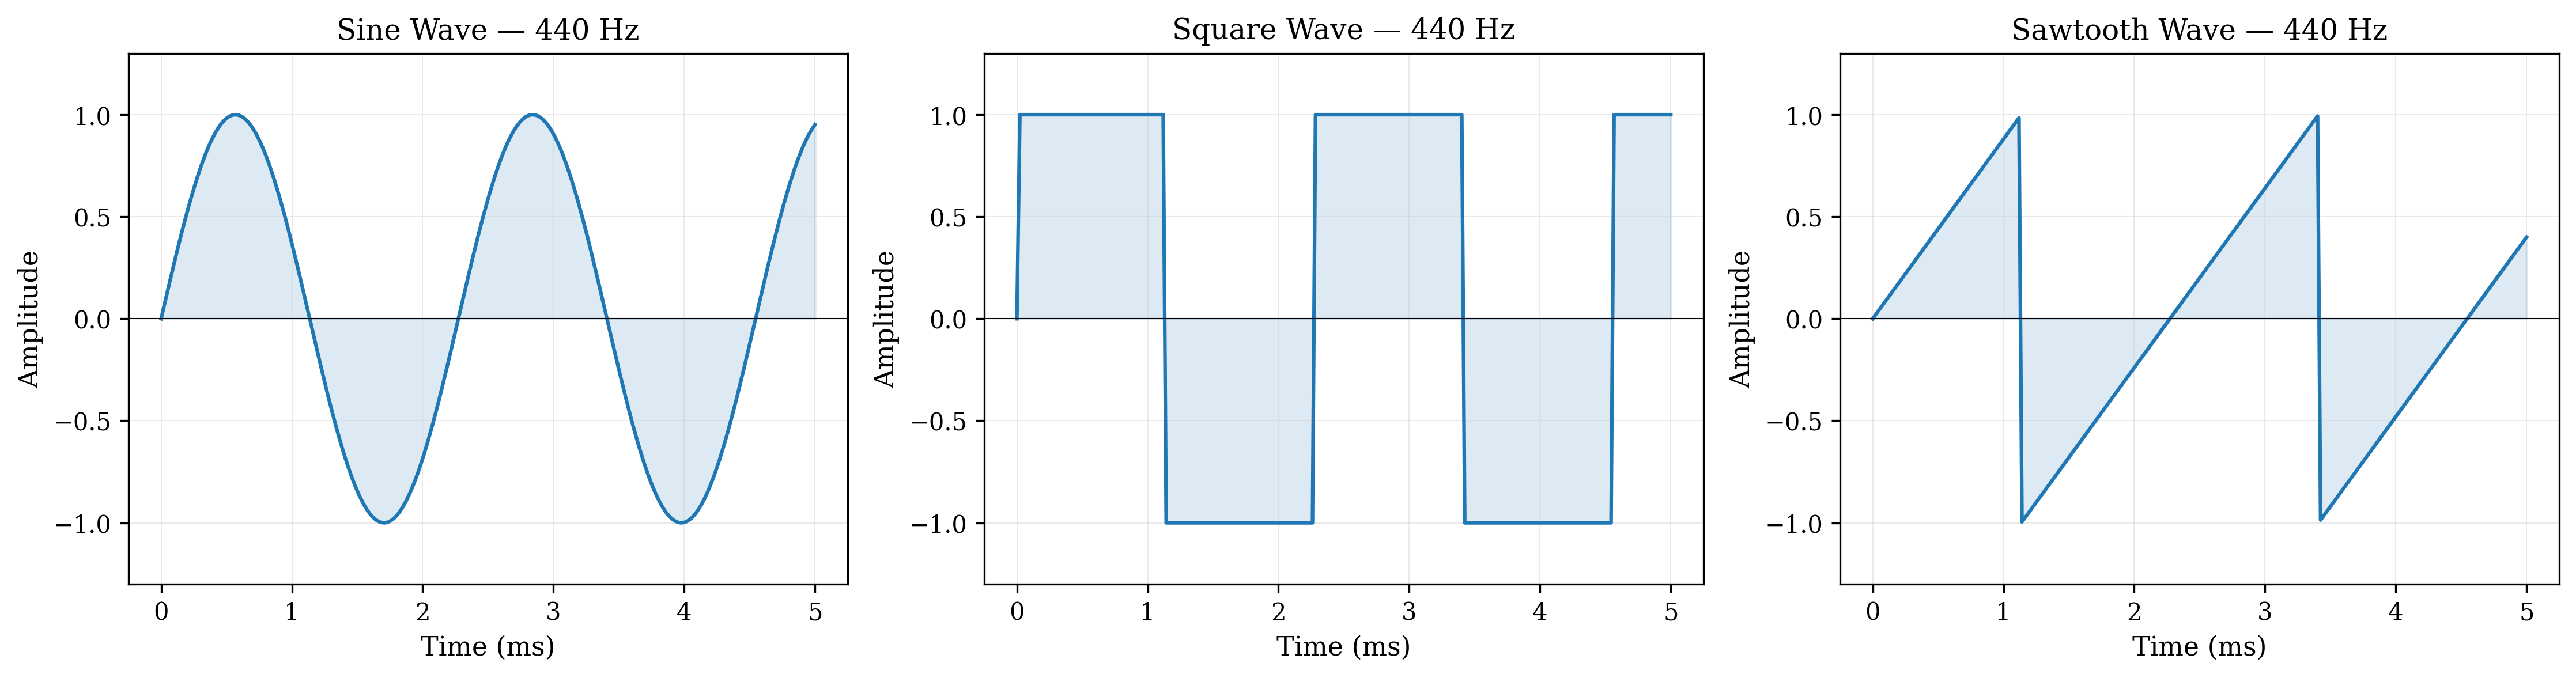
\includegraphics[width=\columnwidth]{figures/waveforms.png}}
\caption{Time-domain waveforms generated by the synthesizer at 440 Hz: sine (left), square (center), and sawtooth (right).}
\label{fig:waveforms}
\end{figure}

The FFT analysis confirms the expected harmonic content: sine (fundamental), square (odd harmonics) and sawtooth (all harmonics decay as $1/n$) \cite{smith2007mathematics}.

\section{Discussion}

\subsection{Strengths}

The HandSynth system demonstrates several notable strengths:

\begin{itemize}
\item \textbf{Accessibility}: Uses a standard webcam, requiring no specialized hardware, depth sensors, or wearable devices.
\item \textbf{Dual-mode configurability}: The rule-based mode provides immediate functionality without any training, while the CNN mode offers improved robustness for users willing to collect a custom dataset.
\item \textbf{Real-time performance}: The system maintains 30 FPS with sub-5 ms CNN inference, providing responsive musical interaction.
\item \textbf{Click-free audio}: Phase-tracked waveform generation eliminates audible artifacts during note transitions.
\item \textbf{Per-hand independence}: The two-hand mapping (melody on right, control on left) enables expressive musical control.
\end{itemize}

\subsection{Limitations}

Limitations include light sensitivity, unclearness of gestures (3 fingers versus 4 fingers), lack of continuous expressiveness (including pitch bend), requirement of user-specific training, and monophonic output.

\subsection{Future Work}

Future work includes continuous gesture, transfer learning, polyphonic synthesis, MIDI output and mobile deployment.

\begin{itemize}
\item Continuous gesture features (e.g., finger spread, hand rotation) for pitch bending and vibrato.
\item Transfer learning from larger hand gesture datasets to reduce the required custom training data.
\item Polyphonic synthesis supporting chord playback.
\item MIDI output for integration with professional digital audio workstations (DAWs).
\item Mobile deployment leveraging TFLite for Android or iOS.
\end{itemize}

\section{Conclusion}

In this paper, HandSynth has been described, a live music synthesizer that is a hand gesture controlled music synthesizer between computer vision and audio synthesis. The system shows that a lightweight CNN (351,558 parameters) with MediaPipe can be responsive with 30 FPS. The two-hand control scheme and dual-mode approach confirm the practicability of vision-based instruments of accessible human-computer interaction.

\section*{Acknowledgment}

The authors would like to thank the faculty and staff of the department for their guidance and support throughout this project.

\begin{thebibliography}{00}
\bibitem{mitra2007gesture} S. Mitra and T. Acharya, ``Gesture recognition: A survey,'' \textit{IEEE Trans. Syst., Man, Cybern. C, Appl. Rev.}, vol. 37, no. 3, pp. 311--324, May 2007.

\bibitem{rautaray2015vision} S. S. Rautaray and A. Agrawal, ``Vision based hand gesture recognition for human computer interaction: A survey,'' \textit{Artif. Intell. Rev.}, vol. 43, no. 1, pp. 1--54, Jan. 2015.

\bibitem{pisharady2015recent} P. K. Pisharady and M. Saerbeck, ``Recent methods and databases in vision-based hand gesture recognition: A review,'' \textit{Comput. Vis. Image Underst.}, vol. 141, pp. 152--165, Dec. 2015.

\bibitem{molchanov2015hand} P. Molchanov, S. Gupta, K. Kim, and J. Kautz, ``Hand gesture recognition with 3D convolutional neural networks,'' in \textit{Proc. IEEE Conf. Comput. Vis. Pattern Recognit. Workshops}, 2015, pp. 1--7.

\bibitem{zhang2020mediapipe} F. Zhang, V. Bazarevsky, A. Vakunov, A. Tkachenka, G. Sung, C.-L. Chang, and M. Grundmann, ``MediaPipe Hands: On-device real-time hand tracking,'' in \textit{Proc. CVPR Workshop on Computer Vision for Augmented and Virtual Reality}, 2020.

\bibitem{paradiso1997electronic} J. A. Paradiso, ``Electronic music: New ways to play,'' \textit{IEEE Spectrum}, vol. 34, no. 12, pp. 18--30, Dec. 1997.

\bibitem{fels1993glove} S. S. Fels and G. E. Hinton, ``Glove-TalkII: A neural-network interface between a data-glove and a speech synthesizer,'' \textit{IEEE Trans. Neural Netw.}, vol. 4, no. 1, pp. 2--8, Jan. 1993.

\bibitem{han2017space} J. Han, G. Shao, D. Leatham, and R. Pasquier, ``Space of sound: A framework for gestural sound control using Kinect,'' in \textit{Proc. Int. Conf. New Interfaces for Musical Expression}, 2017, pp. 345--350.

\bibitem{chowning1973synthesis} J. M. Chowning, ``The synthesis of complex audio spectra by means of frequency modulation,'' \textit{J. Audio Eng. Soc.}, vol. 21, no. 7, pp. 526--534, Sep. 1973.

\bibitem{smith2007mathematics} J. O. Smith, \textit{Mathematics of the Discrete Fourier Transform (DFT) with Audio Applications}, 2nd ed. W3K Publishing, 2007.

\bibitem{tensorflow2015} M. Abadi \textit{et al.}, ``TensorFlow: Large-scale machine learning on heterogeneous systems,'' 2015. [Online]. Available: \url{https://www.tensorflow.org/}

\bibitem{opencv2000} G. Bradski, ``The OpenCV library,'' \textit{Dr. Dobb's J. Softw. Tools}, vol. 25, no. 11, pp. 120--125, Nov. 2000.
\end{thebibliography}

\end{document}